% 01. kapitulua - Hitzaurrea eta helburuak
% Aurreko liburuko hitzaurrearen tonuan: arazoa lehenbizi, abisu zintzoa, bidaiaren pintzelada, helburuak, nola irakurri.
% Lehen pertsona singularrean idatzita; egilekiderik bada, pluralera pasatu (UEUko ebaluatzaileak aurreko liburuan aipatu zuen).
% TODO: 3. paragrafoko eszena generikoa zure benetako esperientzia batekin ordezkatu, aurreko liburuko tesiaren pasadizoak egin zuen moduan.
% Irudiak: Pictures/01/ (goiburu hutsa: header_01.pdf.xoj marraztu eta header_01.pdf.pdf gisa esportatu)

Urte askotan, software-proiektu baten atal astunena kodea idaztea izan da.
Orduak eta orduak teklatuaren aurrean, akatsen bila, funtzionalitate bat amaitu nahian.
Hori bera ikusi izan dugu behin eta berriz Informatika Fakultateko eskoletan: azken egunetako super-heroi kodeketak, presakako integrazioa talde-lanetan eta taldekideen lana balidatzeko edota onartzeko arazoak.
Horregatik idatzi genuen \textit{Git bertsioak kontrolatzeko sistemarako eskuliburua} \parencite{lopezgazpio2024git}: lana ez galtzeko, iterazio inkrementaletan pausoka garatzeko eta taldean integratzeko tresna bat eskura jartzeko.

Egun software-ingeniaritza aldatu da, eta oso azkar, gainera.
Kodetzeko agenteek --hizkuntza-eredu handietan oinarritutako programek, iturburu-kodea idazteko, exekutatzeko eta zuzentzeko gai direnek-- minutu gutxitan egiten dute duela gutxi ikasle bati arratsalde osoa eskatzen zion lana.
Ez dizut gezurrik esango: \textbf{kodea idaztea ez da jada lanik astunena}.
Hala eta guztiz ere, proiektuek lehengo modura porrot egiten jarraitzen dute; batzuetan, akaso, azkarrago.

Har dezagun ohiko kasu bat, adibide gisa.
Lau ikasleko talde batek \textit{sprint} oso bat ``amaitu'' du arratsalde batean, agente bati esker.
Aurkezpenaren egunean demoak huts egiten du.
Inork ez daki azaltzen kodeak zer egiten duen.
Testak pasatzen dira, bai, baina norbaitek --edo zerbaitek-- testak aldatu ditu arazorik egon ez dadin.
Proiektu-taulan dena dago bukatuta egongo balitz modura anotatuta.
Kodea ez zen arazoa, arazoa antolakuntza izan da. Inork ez zituen egin beharrekoak zehaztu, inork ez zuen lana zeregin argitan banatu, eta inork ez zuen egindakoa egiaztatu.

Software-ingeniaritzaren atal kritikoak lekuz aldatu dira: kodea idaztetik, \textbf{zer idatzi erabakitzera}, lana \textbf{zereginetan banatzera}, egindakoa \textbf{egiaztatzera} eta guztia \textbf{integratzera}.
Gaur egun arreta diseinura, koordinaziora eta egiaztapenera bideratu behar da software-ingeniaritza profesionalean (\ref{fig:lan_astunak}~irudia).
Agenteek kodea idazten dute, baina ez dute zure ordez erabakitzen, ez dute zure taldea antolatzen eta ez dira zure lanaren erantzule.
Hori guztia gizakion esku dago, lehen baino gehiago.

% BEHIN-BEHINEKO irudia (matplotlib, xkcd estiloa, Purisa letra); eskuz berriro marrazteko.
\begin{figure}[h]
    \centering
    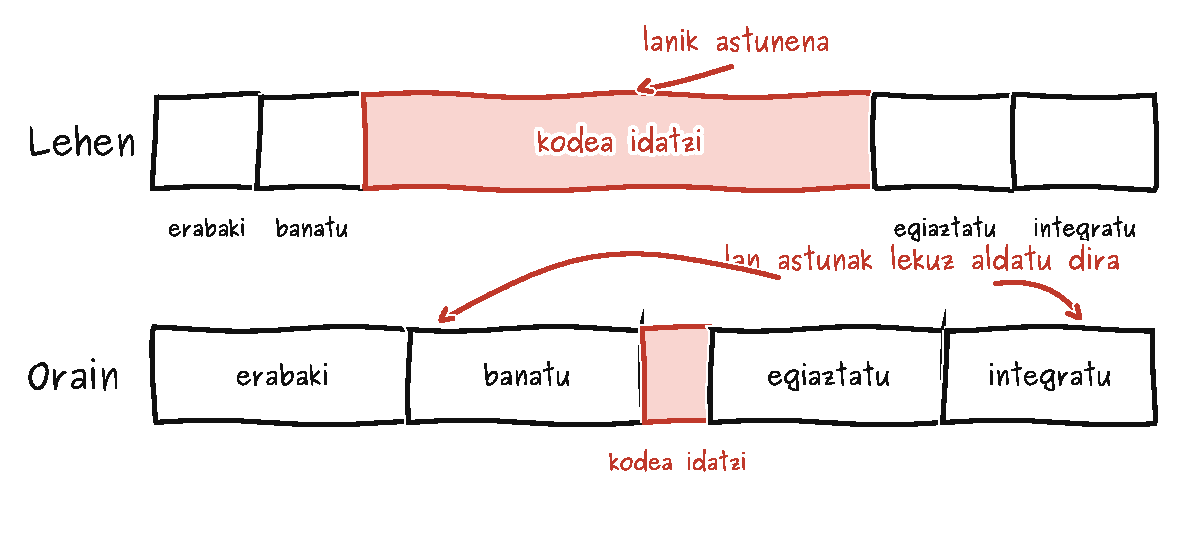
\includegraphics[width=0.95\textwidth]{Pictures/01/1.lan_astunak.pdf}
    \caption{Lan astunak lekuz aldatu dira: lehen kodea idaztea zen lanik astunena; orain erabakitzea, zereginetan banatzea, egiaztatzea eta integratzea dira.}
    \label{fig:lan_astunak}
\end{figure}

Eskuliburu honek \textbf{lantalde hibridoetan} lan egiten irakatsi nahi dizu: gizakiz eta agentez osatutako taldeetan.
Ikusiko duzunez, agenteek lantalde on batek beti behar izan duen gauza bera behar dute, baina zorrotzago: zeregin argiak, onarpen-irizpideak, arauak dituen biltegi bat, epaile gisa jokatzen duen integrazio jarraitua eta berrikuspena.
Agenteak ez du anbiguotasunik barkatzen: zeregin lausoa ematen badiozu, kode okerra idatziko dizu, eta konfiantza osoz gainera.

Ez dizut gezurrik esango, ordea: eskuliburu honek ez zaitu agenteen aditu bihurtuko, eta ez dizu tresna jakin baten erabilera irakatsiko.
Tresnak hilabete gutxitan aldatzen dira, eta liburu hau inprimatzerako batzuk zaharkituta egongo dira.
Horregatik, tresna zehatzak eranskinean eta liburuaren biltegian aipatzen dira, eta liburuan \textbf{aldatzen ez diren kontzeptuak} landuko dira: nola zehaztu, nola antolatu, nola egiaztatu, etab
Eta, Gitekin bezala, hau ere \textbf{erabiliz ikasten da}: bidean ariketa-sorta handia landu beharko duzu, eta ariketa horietako askotan zuk zeuk egingo duzu eskuz gero agenteari emango diozun lana.
Ez dago bestelako misteriorik.

Bada hasieratik aipatu nahi dudan arrisku bat.
Agenteei lana eskuordetzea erraza da; ulermena eskuordetzea, berriz, hondamendia.
Kodea irakurtzen, testak idazten eta arkitektura epaitzen jakin behar duzu, lehen bezainbeste edo gehiago, zuk egiaztatu beharko baituzu agenteak ``eginda'' dioen hori benetan eginda dagoen.
Eskuliburu honek \textbf{ardura} irakatsi nahi du, ez delegazioa.
Ez zaitut agenteak erabiltzera behartu nahi; erabiliko dituzu, nahi ala ez, zure lankideek erabiliko dituztelako.

\section{Nondik gatozen, non gauden}

Eskuliburu honen aurrekari zuzena \textit{Git bertsioak kontrolatzeko sistemarako eskuliburua} da, 2024an UEUk eta UPV/EHUk argitaratua.
Liburu hark hutsune bat bete nahi izan zuen: ez zegoen euskarazko ikasmaterialik bertsioak kontrolatzeko sistemen inguruan, eta Informatika Fakultatean irakasgai askotan erabiltzen da Git.
Git ardatz hartuta, liburuak garapen-metodologiekin, talde-lanarekin eta kode-kalitatearekin lotzen zuen tresna, eta, hain zuzen, lotura horietatik sortu da esku artean duzun liburu hau: nola antolatu software-proiektu handi bat,
nola banatu, nola integratu, etab.

Software-ingeniaritza erabat aldatu da azken urteetan.
Kodetzeko agenteak industrian eta ikasgeletan hedatu dira azkar, eta, hitzaurre honen hasieran esan dudan bezala, lan astunena diseinura, koordinaziora eta egiaztapenera mugitu da.
Horrek esan nahi du software-ingeniaritzaren gaitasun klasikoak --erabiltzaile-historioak, UML, taldeen rolak, metodologia arinak, integrazio jarraitua-- lehen baino beharrezkoagoak direla,
baina lantalde berri baten kontestuan kokatzen dira: gizakiz eta agentez osatutako lantalde hibridoan, hain zuzen ere.

Gaur egun ez dago ikasmaterialik lantalde hibrido horiek antolatzen irakasten duenik, ez euskaraz eta ia ez beste hizkuntzetan ere.
Atzigarri dauden baliabideak bi motatakoak dira: alde batetik, tresna zehatzen dokumentazioa, hilabete gutxitan zaharkitzen dena, eta, bestetik, garapen hibridorako lehen proposamen akademikoak, hala nola \textit{Agentsway} \parencite{bandara2025agentsway}, agenteak taldekide oso gisa hartzen dituena, fase bakoitzerako agente espezializatuekin.
Liburu honen proposamena apalagoa da eta irakasteko egokiagoa: ikasleek dagoeneko ezagutzen dituzten bi metodo hartu --\textit{Scrum} eta \textit{Kanban}-- eta lantalde hibridorako egokitu.
\textbf{Scrumban agentikoa} deritzogu lan egiteko era horri (\ref{cha:scrumban}.~kapitulua): \textit{Scrum}ek gizakien erritmoa antolatzen du --rolak, sprintak, berrikuspena--
eta \textit{Kanban}ek agenteen exekuzioa --zereginen fluxua, lanean dauden atazen mugak, arau esplizituak--.

Egiturari dagokionez, liburu honek aurreko eskuliburuaren bidea jarraitzen du: euskaraz, praktikoa, ariketa ebatziekin eta eskuz egindako irudiekin, errazenetik zailenera.
Eta aurrekoaren osagarria da, ez ordezkoa.

\section{Zer ikasiko dugu}

Jorratuko ditugun gaien pintzelada bat ematearren: hasieran \textbf{taldeez eta rolez} mintzatuko gara (\ref{cha:taldeak}.~kapitulua), Belbinen rolak eta \textit{Scrum}eko rolak gogoratuz, eta agenteak taldean non kokatzen diren erabakiz.
Ondoren, \textbf{erabiltzaile-historioetatik zereginetara} pasatuko gara (\ref{cha:zereginak}.~kapitulua): nola idatzi agente batek --edo taldekide batek-- zalantzarik gabe egikari dezakeen zeregin bat, onarpen-irizpideekin eta egindakoaren definizioarekin.
Jarraian, \textbf{biltegia} lan-eremu partekatu gisa antolatuko dugu (\ref{cha:biltegia}.~kapitulua): zereginaren araberako adarrak, \textit{pull request}-ak, babes-arauak eta integrazio jarraitua epaile gisa izanik.

Teoriarik gabeko kapitulu batean \textbf{eskuak zikinduko ditugu} (\ref{cha:taula}.~kapitulua): proiektu-taula bat sortuko dugu GitHuben, \textit{Kanban} eta \textit{Scrum} ikuspegiak gehituko dizkiogu, \textit{issue}-ak idatzi eta zutabeetan zehar mugituko ditugu, eta \textit{sprint} oso bat simulatuko dugu rol-jokoan.
Hau da, agenteek gero modu automatiko batean kontsumituko duten informazio guztia nola sortzen den eskuz aztertuko dugu.

Behin oinarriak sendo ditugula \textbf{kodetzeko agenteen} inguruan mintzatuko gara (\ref{cha:agenteak}.~kapitulua): zer diren, nola ematen zaien testuingurua, zer baimen behar dituzten, zenbat kostatzen diren eta nola egiten duten huts.
Horren gainean eraikiko dugu liburuaren muina, \textbf{Scrumban agentikoa} (\ref{cha:scrumban}.~kapitulua), metodoaren mekanika osoarekin: nondik datorren izena, zergatik nahasten diren \textit{Scrum} eta \textit{Kanban}, zereginen fluxua, lanean dauden zereginen muga, arau esplizituak eta eskalatze-protokoloa.
Gainbegirale-agente batek, scrumban-agenteak, zainduko du fluxua, eta gizakiak erabakiko ditu garapenaren alderdi kritikoak.

Deskribatu berri dugun fluxua bi ariketa-kapitulutan jarriko dugu praktikan: lehenbizi, \textbf{kaixo, Scrumban agentikoa!} erako ariketa txiki batekin (\ref{cha:kaixo}.~kapitulua) --zeregin bat, agente bat, \textit{pull request} bat--,
eta gero, \textbf{ekosistemaren proiektuarekin} (\ref{cha:ekosistema}.~kapitulua), proiektu konplexu bat agenteen bitartez aurre eginda.
Amaieran, \textbf{DevOps} ikuspegitik egiaztapenaz eta berrikuspenaz arituko gara (\ref{cha:devops}.~kapitulua) --gizakiak zer egiaztatu behar duen, eta nola--, eta \textbf{ohiko arazoen eta errezeten} kapitulu batekin itxiko dugu eskuliburua (\ref{cha:arazoak}.~kapitulua).
Txantiloiak eta konfigurazio-fitxategiak eranskinean bildu ditugu (\ref{cha:eranskina}.~kapitulua).

\section{Helburuak}

Kodetzeko agenteek minutu gutxitan egiten dute duela gutxi garatzaile bati arratsalde osoa lanean jo eta ke lanean egotea eskatuko liokeen kodeketa-lana.
Hala ere, software-proiektuek lehengo modu berean egiten dute porrot.
Lan astunak birmoldatu egin dira: kodea idaztetik zer eraiki erabakitzera, lana zereginetan banatzera, egindakoa egiaztatzera eta integratzera.
Hau da, software-ingeniaritzara.
Eskuliburu honek lantalde hibridoetan (gizakiz eta agentez osatutakoetan) lan egiten irakasteko helburua du: taldeak eta rolak antolatzen, agente batek zalantzarik gabe egikari dezakeen zeregina idazten, biltegia arauekin eta ateekin prestatzen, eta agenteen lana gainbegiratzen eta egiaztatzen.
Muina Scrumban agentikoa da, \textit{Scrum} eta \textit{Kanban} lantalde hibridorako egokitzen dituen lan egiteko modua: \textit{Scrum} gizakien erritmorako, \textit{Kanban} agenteen exekuziorako.
\textit{Git Bertsioak Kontrolatzeko Sistemarako eskuliburua}ren (2024) jarraipena da, egitura eta estilo berarekin: euskaraz, praktikoa, ariketa ebatziekin eta eskuz egindako irudiekin.
Software proiektu handiak bideratzeko kemena duen edonori zuzenduta dago, eta tresnak zaharkitu arren aldatzen ez dena irakatsi nahi du: nola zehaztu, nola antolatu, nola egiaztatu.

Zehazki, eskuliburu hau amaitzean honakoak egiteko gai izatea gustatuko litzaiguke:

\begin{itemize}
    \item agente batek edo taldekide batek anbiguotasunik gabe egikari dezakeen zeregin bat idazteko, onarpen-irizpide eta guzti;
    \vspace{0.15cm}
    \item biltegi bat antolatzeko, zereginaren araberako adarrekin, berrikuspenarekin eta integrazio jarraituarekin;
    \vspace{0.15cm}
    \item proiektu-taula bat kudeatzeko, \textit{Kanban} nahiz \textit{Scrum} ikuspegian;
    \vspace{0.15cm}
    \item agenteen lana gainbegiratzeko Scrumban agentikoaren fluxuan: zereginak esleitu, egoera-txostenak irakurri, blokeoak eskalatu eta lana itxi;
    \vspace{0.15cm}
    \item agente batek egindako lana egiaztatzeko: \textit{diff}-ak irakurri, testak epaitu, arkitektura zaindu;
    \vspace{0.15cm}
    \item agenteen huts egiteko modu ohikoenak antzemateko eta konpontzeko.
\end{itemize}

Eskuliburua edozein programazio-hizkuntzatan kodetzen dakien eta Git erabili duen edonorentzat da.
Giten oinarriak falta bazaizkizu, hasi aurreko eskuliburutik; hemen ez ditugu errepikatuko.
Gogoratu eskuliburu bat ez dela zertan hasieratik bukaerara irakurri behar: taldea antolatzea bada zure larria, hasi \ref{cha:taldeak}.~kapitulutik; agenteekin probatzeko gogoz bazaude, \ref{cha:taula}.~kapituluko ariketak dira abiapuntu ona, \ref{cha:scrumban}.~eta \ref{cha:kaixo}.~kapituluetara salto egin aurretik.
Txantiloiak, konfigurazio-fitxategiak eta ariketen biltegiak liburuaren biltegian daude, eguneratuta.
% TODO: biltegi lagunaren helbidea: \url{...}

Prest zara bideari ekiteko?

\section{Eskerrak}

% TODO: liburua amaitzean idazteko (UEU, zuzentzailea, irakurle goiztiarrak, ikasleak).
\todo[inline]{Eskerrak idazteko, liburua amaitzean.}
